\subsection{Phenotype Extraction}
\label{sec: results phenotype extraction}
\begin{figure}[h]
    \centering
    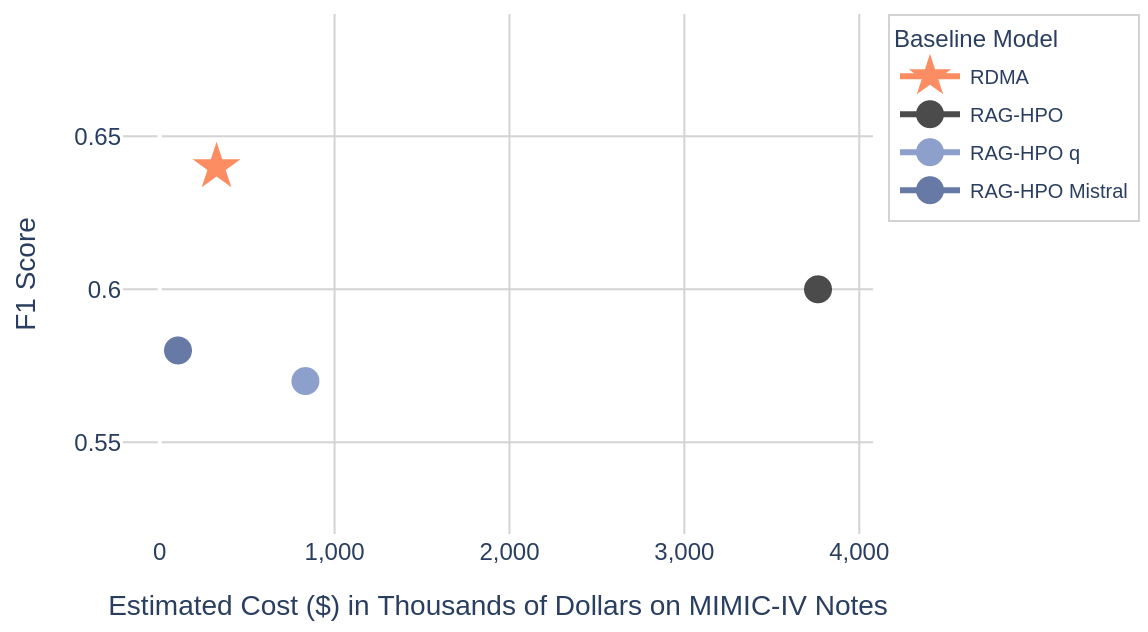
\includegraphics[width=1.0\textwidth]{figs/performance_cost_chart.png}
    \caption{\textbf{RDMA Inference Cost to Performance Compared to RAG-HPO Variants.} RDMA outperforms much more expensive RAG-HPO variants. While RDMA does slightly cost more when accounting for model sizes, the performance benefits are nontrivial. We use GPU rental pricing from cloud-providers \cite{salad_pricing} \cite{hyperstack_gpu_pricing} to compute our inference costs in Appendix \ref{appendix: cost calculations}.}
    \label{fig:performance_cost}
\end{figure}
\textbf{Baselines.} We investigate two rule-based approaches as they are substantially cheaper and easier to run. First, we attempt a simple embedding (MedEmbed \cite{balachandran2024medembed}) retrieval and string matching approach where we retrieve 20 candidates from HPO for each sentence and check if any retrieved entities are mentioned anywhere within the sentence or text. Second, we benchmarked the reported state of the art dictionary-based approach FastHPOCR \cite{groza2024fasthpocr} \cite{garcia2024_HPORAG}. 

\textbf{RAG vs. RDMA.} We compare our approach across a plethora of models between the RAG-HPO and RDMA approaches. For model exploration, we explore biomedically finetuned models such as PhenoGPT \cite{yang2023enhancingphenotyperecognitionclinical}, BERT-based NER i2b2 \cite{rohanian2023lightweight_i2b2}, OpenBioLLM 3 70B \cite{OpenBioLLMs}, and general purpose models such as Llama 3.3 70B \cite{grattafiori2024llama3herdmodels}, Llama 3 70B \cite{grattafiori2024llama3herdmodels}, and the smaller Mistral 24B \cite{mistral2025small}.

\begin{table}[h]
\makebox[\textwidth][c]{% Center the table that's wider than \textwidth
  \resizebox{1.15\textwidth}{!}{% Resize to exactly 1.2\textwidth
    \begin{tabular}{lccccccc}
    \hline
    \textbf{Baseline} & \textbf{Extractor Model} & \textbf{Verifier Model} & \textbf{Matcher Model} & \textbf{Precision} & \textbf{Recall} & \textbf{F1} & \textbf{Local Cost} \\
    \hline
    0-shot & Llama 3.3 70B$^{q}$ & x & x & 0.06 & 0.05 & 0.05 & Medium \\
    \hline
    \multicolumn{8}{c}{\textbf{Rule-based Approaches}} \\
    \hline
    Retrieve and String Match & MedEmbed & x & String Match & 0.60 & 0.21 & 0.31 & Very Low \\
    FastHPOCR & FastHPOCR & x & FastHPOCR & 0.52 & 0.45 & 0.48 & \textbf{Very Low}\\
    \hline
    \multicolumn{8}{c}{\textbf{RAG Approaches}} \\
    \hline
    Stanza RAG-HPO & i2b2 Clinical BERT & x & Llama 3.3 70B$^{q}$ & 0.48 & 0.60 & 0.53 & Medium \\
    Pheno RAG-HPO & PhenoGPT & x & Mistral 24B$^{q}$ & 0.57 & 0.39 & 0.46 & Low \\
    RAG-HPO Mistral & Mistral 24B$^{q}$ & x & Mistral 24B$^{q}$ & 0.55 & 0.61 & 0.58 & Low \\
    RAG-HPO$^{q}$ & Llama 3.3 70B$^{q}$ & x & Llama 3.3 70B$^{q}$ & \textbf{0.65} & 0.56 & 0.60 & Medium \\
    RAG-HPO & Llama 3.3 70B & x & Llama 3.3 70B & 0.59 & 0.55 & 0.57 & High \\
    Bio RAG-HPO & OpenBioLLM 3.3 70B$^{q}$ & x & OpenBioLLM 3.3 70B$^{q}$ & 0.54 & 0.63 & 0.59 & Medium \\
    Cloud RAG-HPO$^{*}$ & Llama 3 70B & x & Llama 3 70B & 0.58 & 0.50 & 0.54 & Cloud \\
    \hline
    \multicolumn{8}{c}{\textbf{RDMA Approaches}} \\
    \hline
    RDMA Bio & Mistral 24B$^{q}$ & OpenBioLLM 3 70B$^{q}$ & Mistral 24B$^{q}$ & 0.52 & 0.70 & 0.60 & Medium \\
    RDMA Large & Mistral 24B$^{q}$ & Llama 3.3 70B$^{q}$ & Mistral 24B$^{q}$ & 0.55 & \textbf{0.70} & \underline{0.62} & Medium \\
    RDMA & Mistral 24B$^{q}$ & Mistral 24B$^{q}$ & Mistral 24B$^{q}$ & \underline{0.63} & \underline{0.68} & \textbf{0.65} & Low \\
    \hline
    \end{tabular}%
  }%
}
\caption{\textbf{Performance of Phenotype Mining Approaches With Respect to Hardware Cost.} $^{q}$Denotes 4-bit quantization. $^{*}$Denotes we were unable to replicate reported performance, but performance is still above non-LLM baselines reported in \cite{garcia2024_HPORAG}. We describe those hardware costs in Table \ref{tab:cost_categories} in Appendix \ref{appendix: cost calculations}. \textbf{Bold} denotes best performance. \underline{Underline} denotes second best.}
\label{tab:model_comparison}
\end{table}

\textbf{Additional reasoning steps with RDMA enables smaller models to outperform much larger models at a fraction of the cost.} Compared to its RAG-based counterparts \cite{garcia2024_HPORAG}, RDMA improves recall performance by over 5\% as shown in Table \ref{tab:model_comparison}, while dramatically reducing upfront operational costs by approximately 4x. Similar to how a clinician reasons when reading clinical notes, these models must go beyond the simple extraction and matching employed in previous phenotype extraction approaches. Specifically, such models must not only extract terms but also verify the accuracy of their extractions and identify implied phenotypes not explicitly mentioned in the text. Fig. \ref{fig:performance_cost} demonstrates that RDMA outperforms all baselines while incurring only minimal additional inference costs for its reasoning steps when compared to similarly-sized RAG-HPO setups using Mistral. One key benefit of moving towards smaller models is that local hardware costs are substantially lower, meaning RDMA is more accessible to a wider range of users. Such costs are key when hospitals must run these tasks locally due to privacy concerns. Please refer to Table \ref{tab:cost_categories} for how we define local hardware costs.

\textbf{Dictionary-based approaches are less comprehensive than LLM-based approaches.} First, we note that almost all LLM approaches outperform the best rule-based approach FastHPOCR \cite{groza2024fasthpocr}, albeit we see that the performance uplift of RAG-HPO is not as extreme as it was reported in \cite{garcia2024_HPORAG}. We hypothesize that the inability to account for contextual information, which is crucial for the correct assignment of HPO codes \cite{gargano2024mode_hpo} to specific entities, leads to subpar performance. Notably, we see that there is almost a 17 \% gap in F1 with an even larger 23\% recall gap between RDMA and FastHPOCR.

\textbf{Large language models can often recognize phenotype text, but cannot directly generate their codes within the ontology.} Within Table \ref{tab:model_comparison}, we see that the zero-shot Llama 3.3 70B has 5\% F1, but its RAG-based matching counterpart has a substantial 60\% F1. Our findings suggest that much of the performance uplift is from the HPO code matching rather than the LLM failing to identify the key pieces within text. In some sense, the zero-shot prediction step taken by the zero-shot model are very similar to the extraction step in the RAG-HPO counterpart, with the only difference being that we ask the zero-shot LLM to generate the HPO code too, which suggests RAG is mainly used to identify the correct codes rather than the text itself. We dig deeper and showcase a comparison where we compare exact code matching to string-based fuzzy matching in Table \ref{tab:exact_vs_fuzzy_metrics} in Appendix \ref{appendix: LLMs are poor ontology code generators}.

\textbf{Fine-tuning leads to worse rare disease-related performance.} In agreement with findings by \cite{wu2024hybrid}, we observe that models explicitly fine-tuned on general medical tasks fail to generalize to more niche rare disease tasks, as shown in Table \ref{tab:model_comparison}. For example, models like OpenBioLLM from \cite{OpenBioLLMs}, despite claiming state-of-the-art performance on common medical benchmarks such as clinician licensing exams, under-perform in rare disease mining. We further discover that fine-tuned PhenoGPT \cite{yang2023enhancingphenotyperecognitionclinical} models as extractors underperform with substantially lower recall compared to their non-fine-tuned counterparts, despite being specifically fine-tuned for phenotype extraction. While this could potentially be attributed to prompting errors, the higher precision suggests these models likely overfit to the BioLarkGSC+ dataset \cite{lobo2017identifying_human_phenotype_terms} used during fine-tuning. Conversely, medically fine-tuned named entity recognition (NER) BERT models such as i2b2 \cite{rohanian2023lightweight_i2b2, qi2020stanza}, specifically designed for extracting mentions of problems (i.e., diseases and conditions) and treatments, exhibit the opposite pattern—achieving much higher recall but often at the cost of noisier extractions, as evidenced by their lower precision. Nevertheless, larger and more general LLMs demonstrate superior performance within both the RDMA and RAG frameworks.

\begin{figure}[h!]
    \centering
    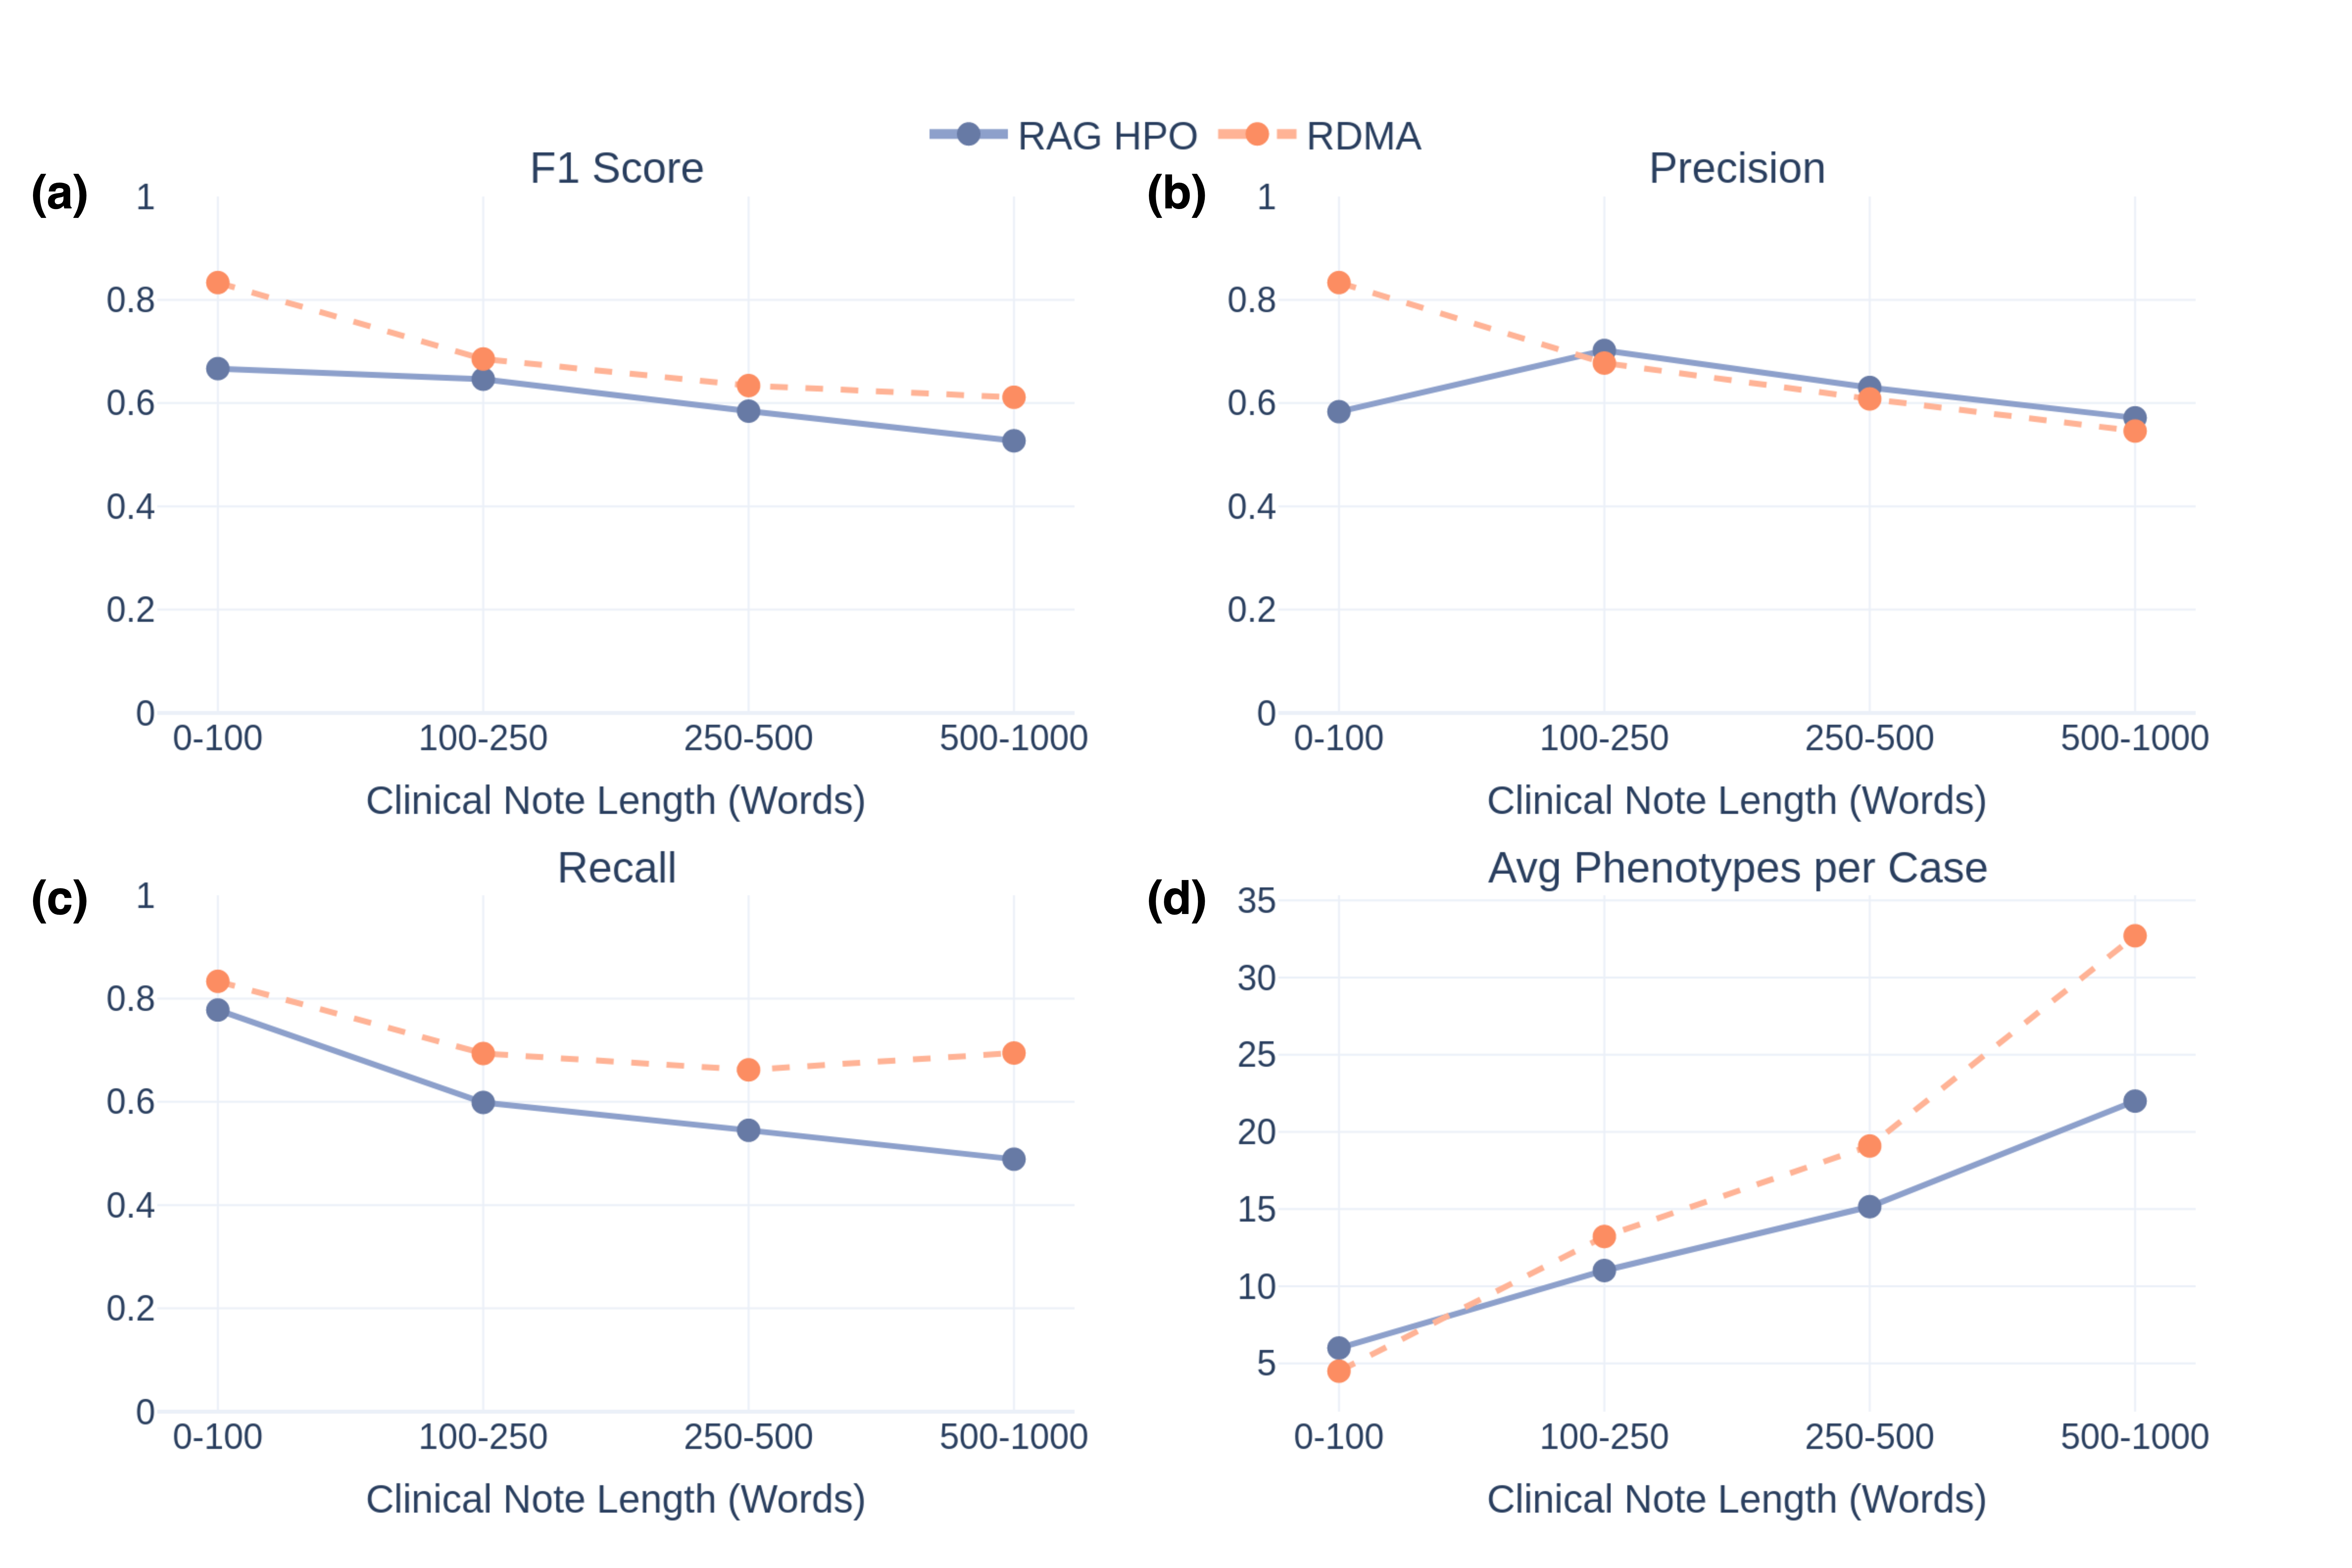
\includegraphics[width=\textwidth]{figs/hpo_metrics_grid_v2.drawio.png}
    \caption{\textbf{RDMA outperforms local RAG-HPO across note lengths.} Real-world clinical notes such as those in MIMIC-IV \cite{johnson2023mimic4_note} are substantially longer than annotated clinical case studies. The median clinical note in MIMIC-IV contains 1,320 words \cite{edin2023automated_medical_coding_survey} compared to 271.5 words in our clinical case study benchmark. Therefore, it is critical that our method maintains reasonable performance across varying note lengths, as the number of phenotypes typically increases with note length (d). While overall precision decreases as note length increases (b), RDMA maintains stable recall performance (c), enabling it to outperform its RAG-based counterpart across all note lengths (a). }
    \label{fig:RDMA_Note_Lengths}
\end{figure}

\textbf{RDMA recall does not degrade as note length increases.} In Fig. \ref{fig:RDMA_Note_Lengths}, we observe that while precision slightly decreases, our overall F1 score appears to flatten out as note lengths increase. Remarkably, our recall slightly increases with longer texts, allowing us to extract more phenotypes as documents grow larger. This suggests that despite some persistent noise (which also affects RAG-HPO approaches), our method demonstrates significantly greater robustness to varying text lengths, ensuring more comprehensive phenotype extraction. We hypothesize this result stems from our approach directly leveraging ontologies within the extraction process—specifically, by retrieving against every sentence and having the LLM agent directly verify whether phenotype-related entities exist within each sentence. In contrast, RAG-HPO approaches typically perform one-shot extraction of the entire document \cite{garcia2024_HPORAG}, explaining why larger models improve performance on these extraction tasks, as increased model size correlates with reduced generation noise \cite{kaplan2020scalinglawsneurallanguage}. Additionally, we instruct our agent to extract anything potentially related to phenotyping, a comprehensive approach not typically employed in RAG-HPO methods.

\begin{table}[htbp]
    \centering
    \begin{tabular}{lccc}
        \toprule
        \textbf{Baseline} & \textbf{F1} & \textbf{Precision} & \textbf{Recall} \\
        \midrule
        RDMA & \textbf{0.651} & 0.626 & 0.678 \\
        RDMA (No Lab Test Tool) & 0.636 & 0.628 & 0.644 \\
        RDMA (No Implication Check) & 0.645 & \textbf{0.640} & 0.650 \\
        RDMA (No verification) & 0.531 & 0.423 & \textbf{0.710} \\
        \bottomrule
    \end{tabular}
    \caption{\textbf{RDMA Ablation Study.} Comparison of performance differences between additional steps that we improve upon the existing RAG HPO \cite{garcia2024_HPORAG} framework.}
    \label{tab:rdma_ablation}
\end{table}

\textbf{What matters in RDMA.} We ablate RDMA by systematically removing several key steps in phenotype extraction, including the lab test tool, phenotype implication reasoning, and the verification step. While performance improvements are observed with each of these components, RDMA sees the most significant improvement from its verification step, which dramatically enhances precision. The other steps primarily contribute to improving the model's recall of additional phenotypes. We further discuss some of its implications and future directions in Section \ref{sec: discussion}.

\begin{figure}[h!]
    \centering
    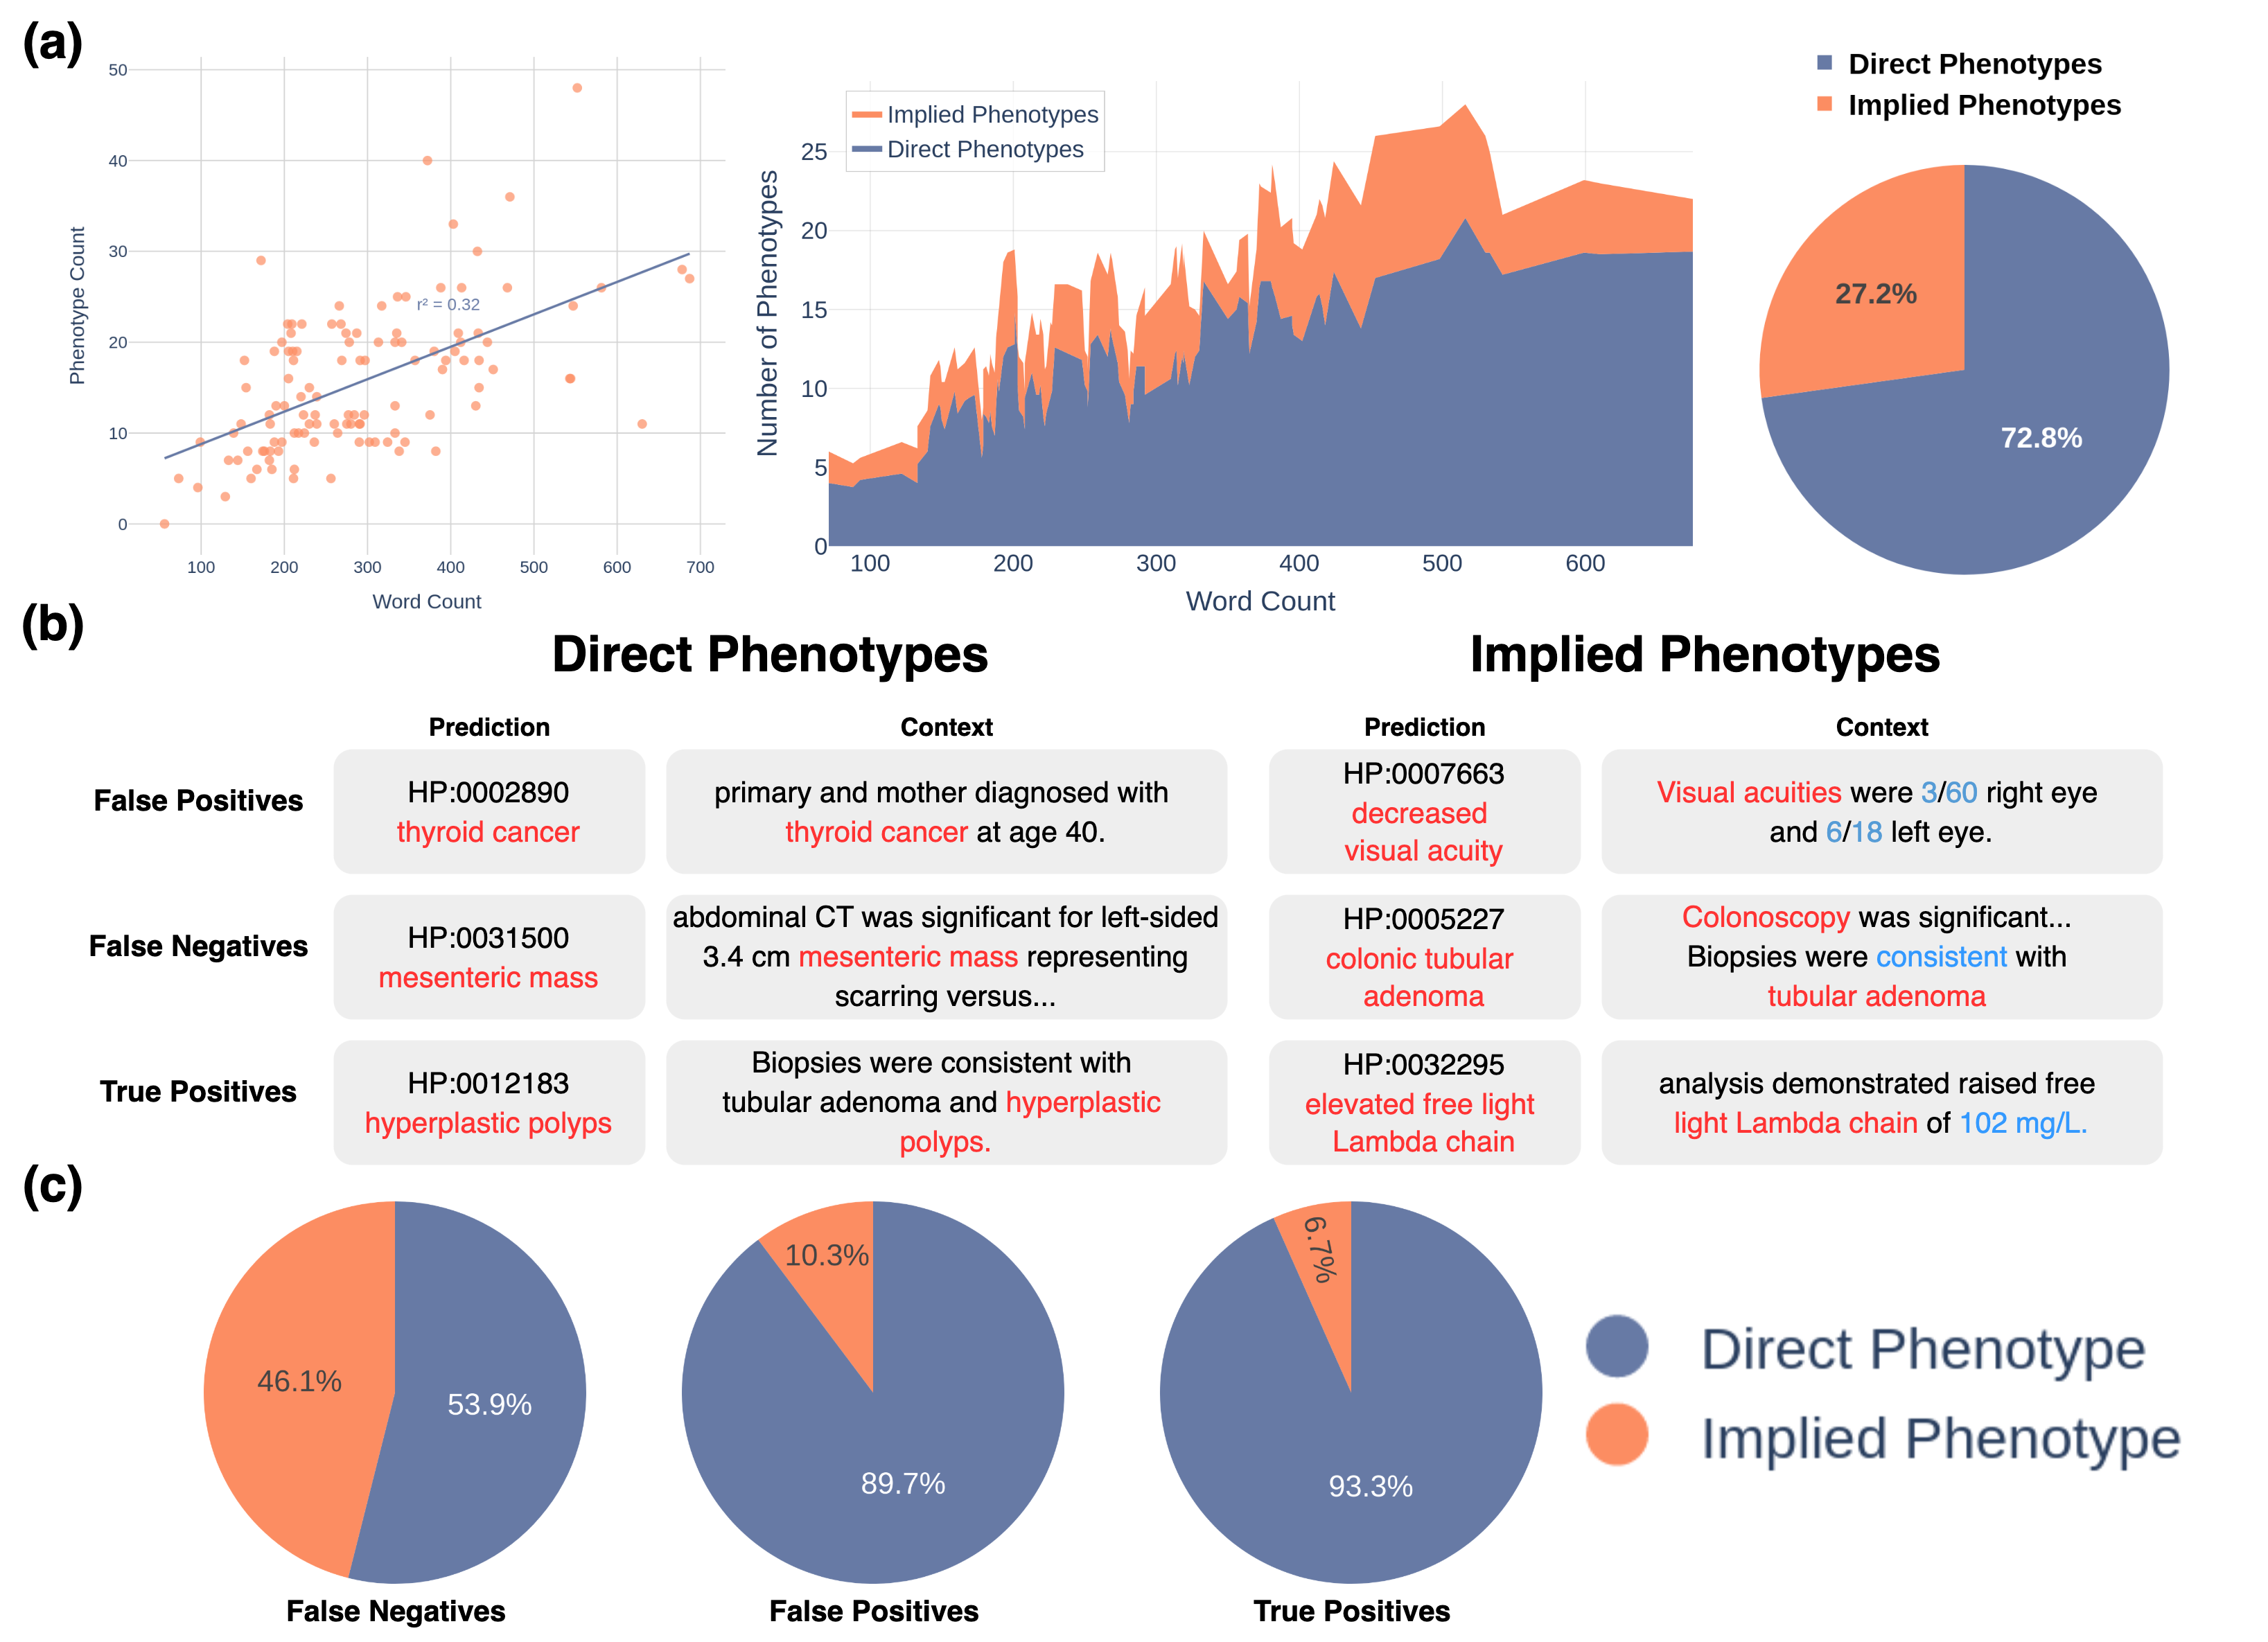
\includegraphics[width=1.0\textwidth]{figs/PhenotypeQualitativeEvaluationsAndStatistics.drawio.png}
    \caption{\textbf{HPO Extraction Evaluation Breakdown.} We evaluate on 116 clinical cases (33,824 words total) from \cite{garcia2024_HPORAG}. \textbf{(a) Dataset Statistics.} Document length weakly correlates with phenotype count. Of 1,813 total phenotypes, 1,320 (72.8\%) appear explicitly in text while 493 (27.2\%) are implied. \textbf{(b) Qualitative Analysis.} Our method captures phenotypes implied by lab tests and related mentions. Key challenges include: (1) False positives that, while not matching labeled HPO codes, are not necessarily incorrect within context—for example, predicting "decreased visual acuity" from impaired vision measurements is clinically valid; (2) False negatives typically arise from missing non-obvious phenotypes like "mesenteric mass" or failing to capture long-range context needed for implied phenotypes like "colonic tubular adenoma," which requires understanding earlier mentions of colonoscopies. Among direct phenotypes, we also observe that there can be cases where the existing label set was not necessarily comprehensive such as "thyroid cancer" not being within the original label set. \textbf{(c) Performance Breakdown.} Though implied phenotypes comprise only 27.2\% of labels, they account for a disproportionate share of false negatives, while most correct predictions are direct phenotypes. }
    \label{fig:DatasetBreakdown}
\end{figure}

\textbf{A substantial number of phenotypes are implied.} Breaking down the benchmark graciously provided by \cite{garcia2024_HPORAG}, their annotations suggest that over 25\% of the phenotypes are not explicitly mentioned in text as shown in Fig. \ref{fig:DatasetBreakdown}. As a key consequence, LLMs need to be able to directly infer such phenotypes from indicators within the text such as lab events and other combinations of symptoms \cite{wei2015extracting_survey_phenotypes}, not obvious in text. We attempt to extract these implied phenotypes through our implication and verification reasoning steps in step 2 in Fig. \ref{fig:RDMAvRAG} with the usage of a lab events range database. However, despite our improvements with the addition of a lab events database tool, its improvement is not dramatic, suggesting that the vast majority of implied phenotypes are still not being caught as shown in Table \ref{tab:rdma_ablation}. This large presence of implied phenotypes could also explain why all baselines struggle to surpass 65 \% F1 in phenotype extraction.

\textbf{Clear Challenges in Mining Phenotypes.} To better understand the sources of error, we examine false positive and false negative cases for our phenotypes in Fig. \ref{fig:DatasetBreakdown} (b). Many false positives are not technically incorrect despite lacking the exact code from human annotations. For example, "decreased visual acuity" correctly reflects the eye measurements but does not precisely match the manually annotated HPO code "reduced visual acuity." Conversely, RDMA sometimes identifies direct phenotypes like "thyroid cancer" that human annotators missed, suggesting our method can capture entities overlooked during manual annotation. However, RDMA frequently fails to extract phenotypes that require long-context reasoning or inference from implicit information. This performance gap indicates that agentic systems still face challenges in identifying implied phenotypes. Despite these limitations, our relative performance metrics across all methods align with our brief qualitative observations.